\documentclass[border=2]{standalone}
\usepackage{tikz}

\usetikzlibrary{shapes,arrows,arrows.meta,fit,positioning}

\begin{document}
\begin{tikzpicture}
    \node at (0,0) (A) {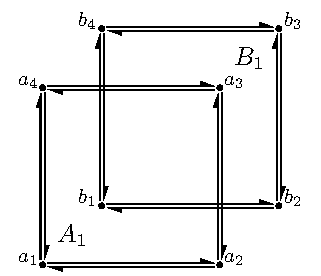
\includegraphics[page=1]{dcel1}};
    \node[right = -0.1 of A] (B) {\includegraphics[page=2]{dcel1}};
    \node[right = -0.1 of B] (C) {\includegraphics[page=3]{dcel1}};
    \draw[thick, -latex] (2.25,0) -- (3.00,0);
    \draw[thick, -latex] (7.25,0) -- (8.00,0);
\end{tikzpicture}
\end{document}
